\section{Locally Linear Embedding (LLE)}

\mode<presentation>{
\begin{frame} 
    \begin{center} \huge
        \secname
    \end{center}
\end{frame}
}

\subsection{Motivation}

\begin{frame}{\subsecname}

Find structure in the data that extends to non-linear manifolds.

\notesonly{

$\textbf{S}$-dataset provides an example of a non-linear manifold.}

\begin{figure}[ht]
	\centering
    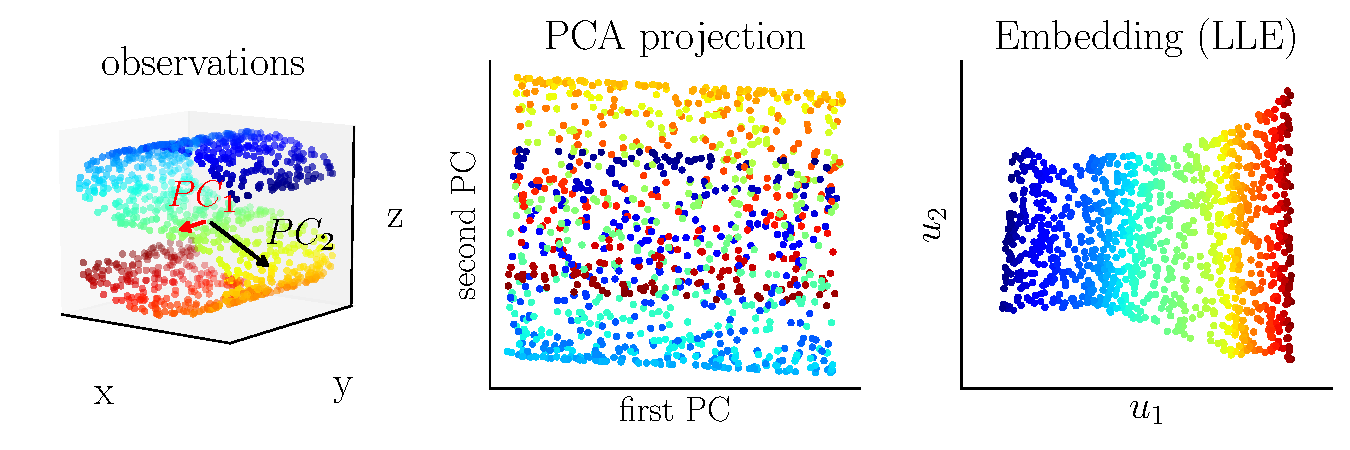
\includegraphics[width=12cm]{img/s_data_proj}
	\notesonly{\caption{The S-dataset, PCA projections and embedding solution. Points are colorized according to their index in the dataset.}}
	\label{fig:s_data_proj_lle}
\end{figure}

\notesonly{
Utilize this to r}\slidesonly{R}educe the dimensionality of the data such that points that lie close \textbf{on} the manifold also lie close in their projection\notesonly{ (we will refer to the projection space which preserving local neighborhoods / ``structure preserving'' as \emph{embedding space})}.

\end{frame}

\notesonly{
Looking at \figref{fig:s_data_proj_lle} we see that the nonlinear manifold is preserved in the LLE embedding, while PCA does not capture the non-linear local structure. The same can be said for \figref{fig:faces_translated_pca_lle}, translating the images from one corner to another has a corresponding translation in the embedded space. In this case we can also infer the coordinates of an image where the face appears in the bottom-left corner in the embedded space.
}

\begin{frame}
\slidesonly{
 \frametitle{Locally Linear Embedding (LLE)}
}
 
\begin{figure}[ht]
	\centering
    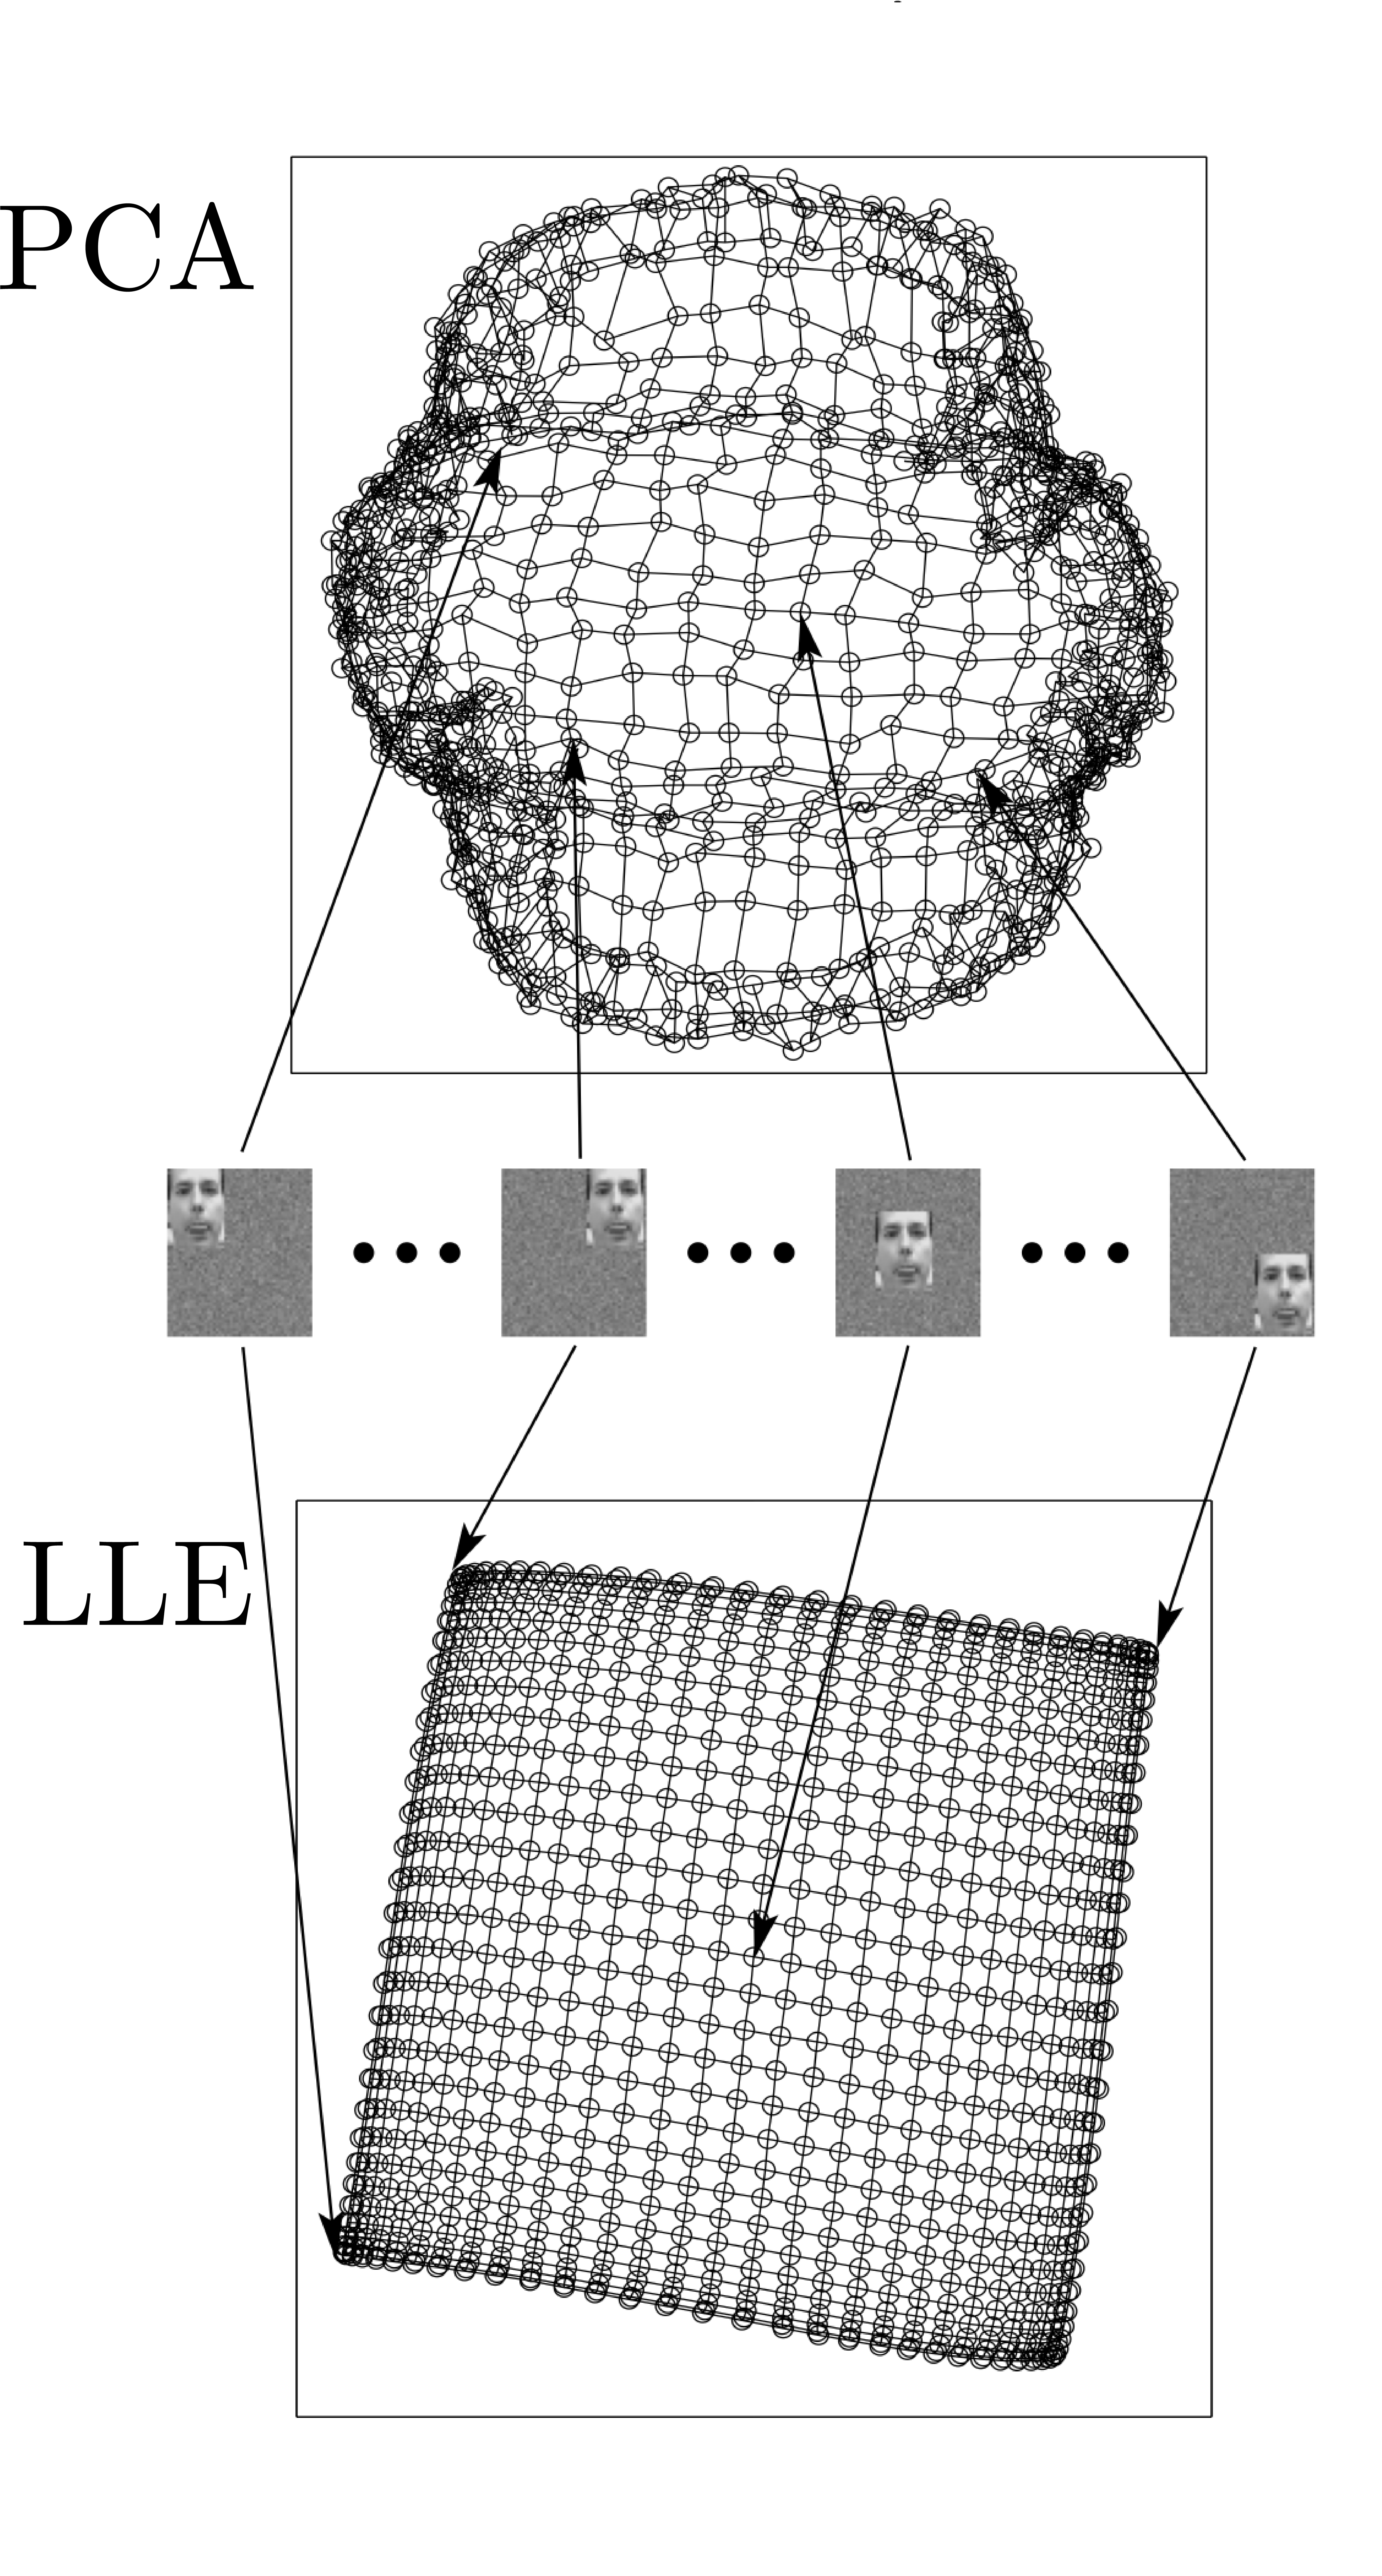
\includegraphics[width=0.3\textwidth]{img/fig3_lle_intro_cropped.png}
	\caption{PCA projections and LLE of translated versions of the same image. What would be the coordinates of the face-in-bottom-left-corner-image be?}
	\label{fig:faces_translated_pca_lle}
\end{figure}
\end{frame}

\subsection{The algorithm}

\subsubsection{A representation of local structure}

\begin{frame}{\subsecname:~\subsubsecname}

\notesonly{
LLE is a fairly simple algorithm. }Local structure is preserved by optimizing the projection of a neighborhood of points (PCA finds a projection for all points collectively).

\pause

But first we have to identify the neighborhood.

\end{frame}

\begin{frame}{\subsecname:~\subsubsecname}

\question{How do we ``localize'' the local structure?}

\pause

- through K-nearest neighbors

\begin{figure}[ht]
	\centering
    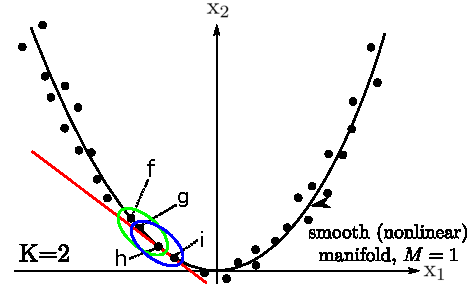
\includegraphics[width=8cm]{img/section4_fig11_K2}
	\label{fig:tangentialk2}
\end{figure}

\end{frame}

\begin{frame}
\textbf{switch to lecture slides}

\end{frame}

\begin{frame}{Step 2: calculate reconstruction weights}
\begin{equation}
E(\vec{W}) = \sum_{\alpha=1}^{p} \underbrace{\lVert\vec{x}^{(\alpha)} - \sum_{\beta=1}^{p} \mathrm{W}_{\alpha \beta} \vec{x}^{(\beta)}\rVert^2}_{
\substack{=e^{(\alpha)}\\\text{reconstruct } \vec{x}^{(\alpha)} \text{ by its } \\ K \text{ nearest neighbors only}}
}
\eqexcl \min_{\vec W}
\end{equation}
\begin{equation}
\text{s.t.} \quad \mathrm{W}_{\alpha \beta} = 0 \text{ if } \beta \notin \operatorname{KNN}(\vec{x}^{(\alpha)}), \qquad
\sum_{\beta=1}^{p} \mathrm{W}_{\alpha \beta} = 1
\end{equation}\\

for each data point $\vec{x}^{(\alpha)}$ (result from applying Lagrange multiplier method):
\begin{itemize}
	\item local ``covariance'' matrix (symmetric \& positive semidefinite) $\vec{C}^{(\alpha)} \in \mathbb{R}^{K,K}:$ 
\end{itemize}

\end{frame}

\begin{frame}
\slidesonly{\frametitle{Step 2: calculate reconstruction weights (cont'd)}}

\slidesonly{
\begin{equation}
\mathrm{W}_{\alpha \beta} = 0 \text{ if } \beta \notin \operatorname{KNN}(\vec{x}^{(\alpha)}), \qquad
\sum_{\beta=1}^{p} \mathrm{W}_{\alpha \beta} = 1
\end{equation}
}

\begin{align}
e^{(\alpha)} &= \lVert\vec{x}^{(\alpha)} - \sum_{\beta=1}^{p} \mathrm{W}_{\alpha \beta} \vec{x}^{(\beta)}\rVert^2\\
&\stackrel{\text{sum to 1 for} \beta \in \text{KNN}}{=} \lVert \sum_{\beta=1}^{p} \mathrm{W}_{\alpha \beta} \vec{x}^{(\alpha)} - \sum_{\beta=1}^{p} \mathrm{W}_{\alpha \beta} \vec{x}^{(\beta)}\rVert^2\\
\end{align}/

\textbf{switch to LLE lecture slides}

\end{frame}

\begin{frame}%[label=g_alpha_beta_proof]{Supplementary Material}
%\begin{textblock}{5}(13,0.075)
	%\hyperlink{g_alpha_beta_slide}{\beamerbutton{back to lecture}}
%\end{textblock}
	Derivation of $g_{\alpha \beta}$ in the cost function
	$F(\vec U) =
    \sum_{\alpha=1}^{p} 
	\bigg(  \vec{u}^{(\alpha)}  - \sum_{\beta=1}^{p} W_{\alpha \beta} \vec{u}^{(\beta)}
	\bigg) ^ 2
    $ 
    for finding the optimal embedding coordinates.\\
    First, a brief refresher on binomial expansion of vectors:
	%{\footnotesize{}
    \begin{align}
    \big( 
		\vec{a}
		- \vec{b}
	\big) ^ 2 
    &= \big(  \vec{a} - {\color{blue}\vec{b}} \big)^\top \big(  \vec{a} - {\color{red}\vec{b}} \big)\\
    &= \vec a^\top \vec a 
    - \vec a^\top {\color{red}\vec{b}}
    - {\color{blue}\vec{b}^\top} \vec a 
    - {\color{blue}\vec{b}^\top} {\color{red}\vec{b}}
    \end{align}\\
    
    Let $\;\vec a = \vec u^{(\alpha)}\;$ and 
    $\;{\color{red}
    \vec{b}=\sum_{\beta=1}^{p} W_{\alpha \beta} \vec{u}^{(\beta)}
    } \Leftrightarrow {\color{blue}
    \vec{b}^{\top}=\sum_{\beta=1}^{p} 
    W_{\beta \alpha} \left(\vec{u}^{(\beta)}\right)^\top
    }
    $
    
    \question{Why do we flip the indices from 
    ${\color{red} W_{\alpha \beta}}$ to ${\color{blue} W_{\beta \alpha}}$?}\\
    The reason we flip the Transposing $\vec u^{(\beta)}$ 
    
    \begin{align}
	= &\sum_{\alpha=1}^{p} 
	\bigg[ 
	(\vec{u}^{(\alpha)})^2
	- 2 \sum_{\beta=1}^{p} W_{\alpha \beta} (\vec{u}^{(\alpha)} )^\top \vec{u}^{(\beta)}
	+
	\sum_{\beta=1, \gamma=1}^{p} W_{\alpha \beta} W_{\alpha \gamma} (\vec{u}^{(\beta)} )^\top \vec{u}^{(\gamma)}
	\bigg]
	\\
	= &\sum_{\alpha=1}^{p} 
	\bigg[ 
	(\vec{u}^{(\alpha)})^2
	- \sum_{\beta=1}^{p} W_{\alpha \beta} (\vec{u}^{(\alpha)} )^\top \vec{u}^{(\beta)}
	- \sum_{\beta=1}^{p} W_{\beta \alpha} (\vec{u}^{(\beta)} )^\top \vec{u}^{(\alpha)}
	\\~~~~~~~&+
	\sum_{\beta=1}^{p} 
		\sum_{\gamma=1}^{p} 
		\bigg(
			W_{\gamma \alpha} 
			W_{ \gamma \beta}
		\bigg) 
		(\vec{u}^{(\alpha)} )^\top \vec{u}^{(\beta)}
	\bigg]
	\\
	= &\sum_{\alpha, \beta=1}^{p} 
	\bigg\{ \underbrace{
		\delta_{\alpha \beta}
		- W_{\alpha \beta}
		- W_{\beta \alpha}
		+
		\sum_{\gamma=1}^{p} 
			W_{\gamma \alpha} W_{\gamma \beta} }_{=g_{\alpha \beta}}
	\bigg\}
	(\vec{u}^{(\alpha)} )^\top \vec{u}^{(\beta)}
	\end{align}
    %}
\end{frame}
